\exer{Exercice d'application}


On considère le graphe \texttt{G} suivant, où le nombre situé sur l'arête joignant deux sommets est leur distance, supposée entière :
\begin{center}
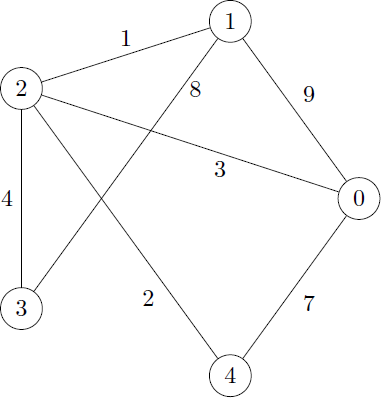
\includegraphics[width=.75\linewidth]{02_application}
\end{center}


\question{Construire la matrice $\left( M_{ij}\right)_{0\leq i,j\leq 4}$, matrice de distances du graphe \texttt{G}, définie par :
<< pour tous les indices $i$, $j$, $M_{ij}$ représente la distance entre les sommets $i$ et $j$,
ou encore la longueur de l'arête reliant les sommets $i$ et $j$ >>.}

On convient que, lorsque les sommets ne sont pas reliés, cette distance vaut $-1$. La distance du
sommet $i$ à lui-même estégale à 0.
\question{Écrire une suite d'instructions permettant de dresser à partir de la matrice \texttt{M} la liste des voisins du sommet 4.}

\question{Écrire une fonction \texttt{voisins}, d'argument un sommet $i$, renvoyant la liste des voisins du sommet $i$.}

\question{Écrire une fonction \texttt{degre}, d'argument un sommet $i$, renvoyant le nombre des voisins du sommet $i$, c'est-à-dire le nombre d’arêtes issues de $i$.}

\question{Écrire une fonction \texttt{longueur}, d’argument une liste \texttt{L} de sommets de \texttt{G}, renvoyant la longueur du trajet d'écrit par cette liste \texttt{L}, c’est-à-dire la somme des longueurs des arêtes empruntées. Si le trajet n'est pas possible, la fonction renverra $-1$.}
